\documentclass{cernatsnote}
\usepackage{physics}

\usepackage{tcolorbox}
\tcbuselibrary{skins}
\usepackage{lipsum}
\usepackage{mathtools}
\usepackage{amsfonts}
\usepackage[colorinlistoftodos]{todonotes}
\usepackage{placeins}
\usepackage{amsmath}
\usepackage{physics}
\usepackage{tcolorbox}
\tcbuselibrary{skins}
\usepackage{lipsum}
\usepackage{amsmath}
\usepackage[T1]{fontenc}
\usepackage{graphicx, subfigure}
\usepackage{fancyhdr}
\usepackage{lmodern}
\usepackage{color}
\usepackage{transparent}
\usepackage{amsfonts}
\usepackage{mathtools}
\usepackage{tikz}
\usetikzlibrary{positioning}
\usepackage{pgfplots}
\pgfplotsset{compat=1.10}
\usepackage{textcomp}
\usepackage{float}
\usepackage{adjustbox} % Used to constrain images to a maximum size 
\usepackage{color} % Allow colors to be defined
\usepackage{enumerate} % Needed for markdown enumerations to work
\usepackage{geometry} % Used to adjust the document margins
\usepackage{amsmath} % Equations
\usepackage{amssymb}
\usepackage{fancyvrb} % verbatim replacement that allows latex
\usepackage{grffile} % extends the file name processing of package graphics 
                         % to support a larger range 
    % The hyperref package gives us a pdf with properly built
    % internal navigation ('pdf bookmarks' for the table of contents,
    % internal cross-reference links, web links for URLs, etc.)
\usepackage{hyperref}
\usepackage{longtable} % longtable support required by pandoc >1.10
\usepackage{tabularx}
\usepackage{epigraph}
\usepackage{quotchap}
\usepackage{lscape}
\usepackage{enumerate}
\usepackage{xpatch}
\usepackage{titletoc}
\usepackage{float}	
\usepackage{xparse}
\NewDocumentCommand{\DIV}{om}{%
  \IfValueT{#1}{\setcounter{#2}{\numexpr#1-1\relax}}%
  \csname #2\endcsname
}

%\renewcommand{\thesubsection}{\thesection.\alph{subsection}}


\title{Computational Physics – Exercise 2}
\author{Pugazharasu Anancia Devaneyan, Rishi Kumar Senthil Kumar}
\email{\href{pugs@uni-bonn.de}{pugs@uni-bonn.de}, \href{s6risent@uni-bonn.de}{s6risent@uni-bonn.de}}
\date{\today}

\begin{document}
\maketitle

%\begin{abstract}
%This document summarizes ideas from Group theory and representation theory that are vital for the upcoming seminar.
%\end{abstract}
%\\ \\ \\ 

%\begingroup
%\color{black}
%\tableofcontents
%\endgroup

%\section*{Test}
%\section*{Simulation of the 1-D Ising model}
\section{Simulating the Ising model in $d=2$}
We simulated the Ising model in $d=2$, the code can be found at \cite{github}.

\section{Numerical cost of the calculation of the energy}
We know that calculating the energy of a given spin configuration involves summing over all the sites, thus the numerical cost of calculating the energy is  $\mathcal{O}(\Lambda)$ for $\Lambda = N_{x} \times N_{y}$ or $\mathcal{O}(N^{2})$ for $N = N_{x} = N_{y}$.
\section{Numerical cost of the calculation of the change in energy}
We know that to calculate the change in energy of a spin update, we only need to consider neighbouring spins which depends on dimensionality $d$ for $N_{x} = N_{y}$ and not on the system size $\Lambda$, thus the numerical cost of calculating the change in energy is  $\mathcal{O}(\lambda)$ where $\lambda$ is some constant independent of system size.
\section{Significance of the critical coupling}
The critical coupling is point at which the average magnetization vanishes. We observer a phase transition at that point \cite{thijssen}.
\section{Estimating the average magnetization per site}
We can estimate the average magnetization per site, $\langle m \rangle$ as a function of $J \in [-1,1]$ while we hold $J = 0.5$ and $N \in [2,4,6,8,10,12,14,16,18,20]$
\begin{figure}[H]
    \centering
    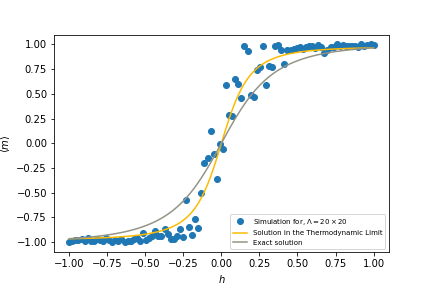
\includegraphics[scale = 0.7]{images/m_v_h_20.png}
    \caption{A plot of the average magnetization per site $\langle m \rangle$, as a function of $h$ for $N = N_{x} = N_{y} = 20$ sites}
    \label{fig:avg_mag}
\end{figure}
\section{Estimating the average energy per site}
We can estimate the average energy per site, $\langle \epsilon \rangle$ as a function of $J^{-1}, \forall J \in [0.25,2]$ while we hold $h = 0$ and $N \in [2,4,6,8,10,12,14,16,18,20]$
\begin{figure}[H]
    \centering
    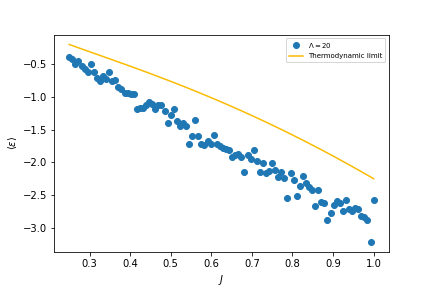
\includegraphics[scale = 0.5]{images/e_v_j_20.png}
    \caption{A plot of the average magnetization per site $\langle m \rangle$, as a function of $h$ for $N = N_{x} = N_{y} = 20$ sites}
    \label{fig:e_v_j}
\end{figure}
The simulation comes close to displaying the qualitative behaviour of what we observe in the thermodynamic limit however there is a quantitative difference, we expect this to disappear as $N$ becomes larger.
\section{Estimating the absolute value of the mean magnetization}
We plot for absolute value of the mean magnetization, $\langle | m | \rangle$ the versus the reciprocal of the nearest neighbour coupling, $J^{-1} \in [0.25,1]$ in figure \ref{fig:abs_mag}. We observe a drop in absolute magnetization as predicted at
\begin{equation}
    J_c=\frac{1}{2} \log (1+\sqrt{2}) \approx 0.440686793509772
\end{equation}
\begin{figure}[H]
    \centering
    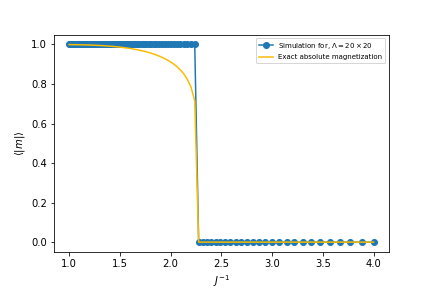
\includegraphics[scale = 0.6]{images/abs_m_v_J_20.png}
    \caption{A plot of the average absolute magnetization per site $\langle | m | \rangle$, as a function of $J^{-1}$ for $N = N_{x} = N_{y} = 20$ sites.}
    \label{fig:abs_mag}
\end{figure}
Moreover, the simulation misses this phase transition's shape and displays a sharp drop, we expected this as we know that the Hasting's algorithm is not effect near critical points.
However, when we plot for mean magnetization versus the reciprocal of the nearest neighbour coupling, $J^{-1}$ as shown in figure \ref{fig:mag_v_j}, we completely miss out on the phase transition.
\begin{figure}[H]
    \centering
    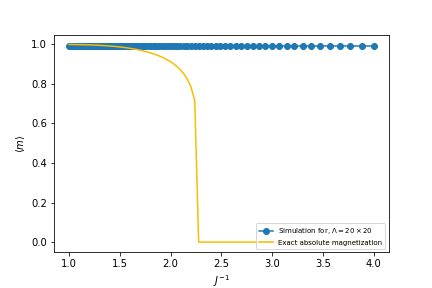
\includegraphics[scale = 0.6]{images/m_v_j_20.png}
    \caption{A plot of the average magnetization per site $\langle m \rangle$, as a function of $J^{-1}$ for $N = N_{x} = N_{y} = 20$ sites.}
    \label{fig:mag_v_j}
\end{figure}
\section{Computing the specific heat}
Specific heat is given by,
\begin{equation}
    C=\Lambda *\left(\left\langle\epsilon^2\right\rangle-\langle\epsilon\rangle^2\right)
\end{equation}
and in the thermodynamic limit
\begin{equation}
    C=\frac{4 J^2}{\pi \tanh ^2(2 J)}\left(K\left(\kappa^2\right)-E\left(\kappa^2\right)-\left(1-\tanh ^2(2 J)\right)\left[\frac{\pi}{2}+\left(2 \tanh ^2(2 J)-1\right) K\left(\kappa^2\right)\right]\right)
\end{equation}
where $K(m)$ and $E(m)$ are the incomplete elliptic integral of the first and second kind, respectively, and
\begin{equation}
    \kappa=\frac{2 \sinh (2 J)}{\cosh ^2(2 J)}
\end{equation}
Here we plot figure \ref{fig:c_v_j} for $C/J^{2}$ as function $J^{-1}$ for $J \in [0.25,1]$ and 
\begin{figure}[H]
    \centering
    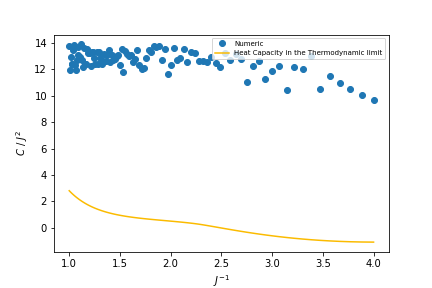
\includegraphics[scale = 0.7]{images/c_v_j_20.png}
    \caption{A plot of the scaled specific heat $C/J^{2}$, as a function of $J^{-1}$ for $N = N_{x} = N_{y} = 20$ sites.}
    \label{fig:c_v_j}
\end{figure}
Although there is a quantitative difference by at least an order of of a magnitude. After some trial and error, we found that this factor is independent of $N$. However, if we were to subtract a constant ($10$ in our case) we obtained the following plot.
\begin{figure}[H]
    \centering
    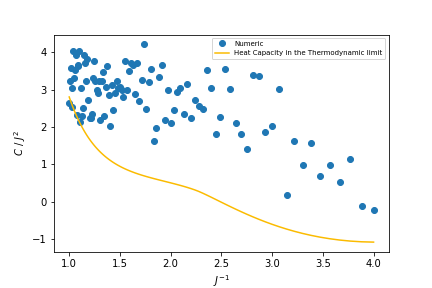
\includegraphics[scale = 0.7]{images/c_v_j_corr.png}
    \caption{The plot we obtain after subtracting a constant from $C/J^{2}$ in figure \ref{fig:c_v_j}}
    \label{fig:correction}
\end{figure}
We think that this due to us not having a perfect Markov chain i.e. presence of correlations. In the lecture, a "autocorrelation" correction was mentioned as the cure for this. However, we were unable to find it.
\bibliographystyle{abbrv}
\bibliography{Bibliography.bib}
\end{document}